% !TeX root = ../main.tex
% Add the above to each chapter to make compiling the PDF easier in some editors.

\chapter{Weight-Space Learning}\label{section:wsl}

\begin{figure}[h!]
    \centering
    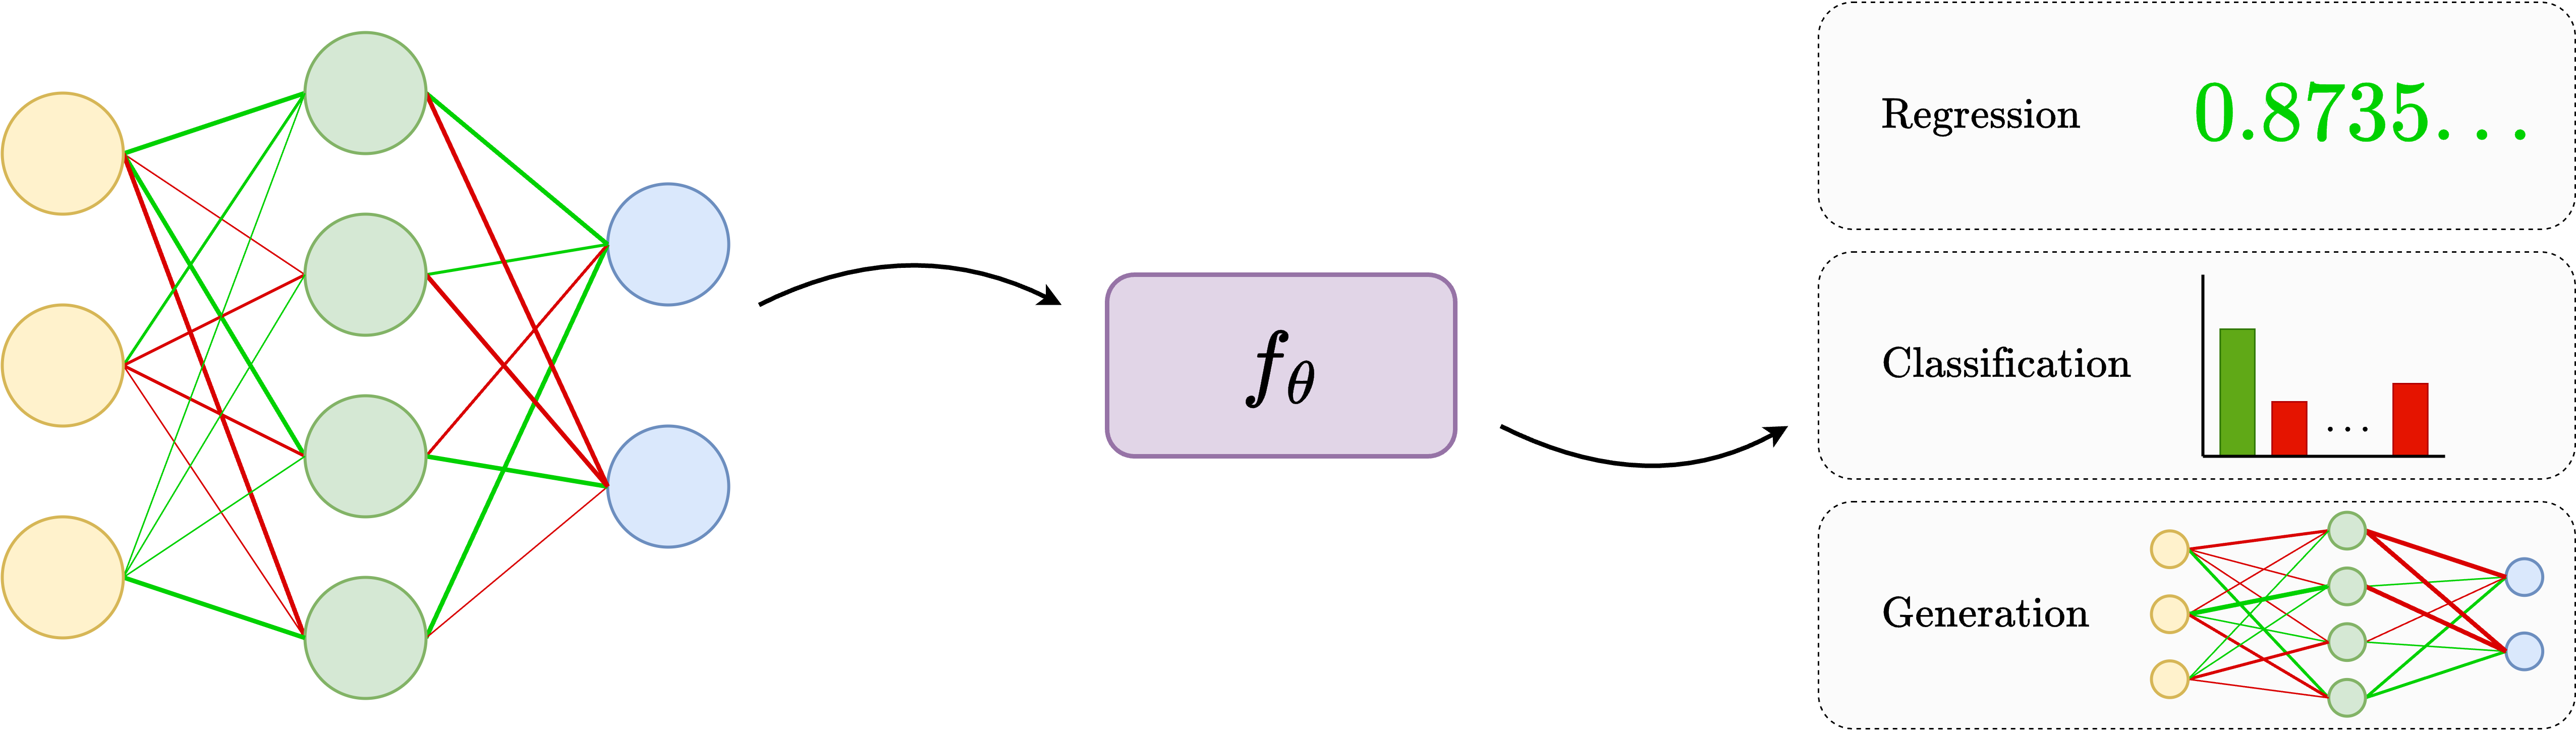
\includegraphics[width=0.8\linewidth]{figures/wsl.drawio.png}
    \caption{\label{fig:wsl} Weight-space learning}    
\end{figure}

Training neural networks on other neural networks' weights has been an active research area for a long time \citep{haHyperNetworks2016, kruegerBayesianHypernetworks2018}, but has seen increasing interest recently with new neural network architectures being proposed \citep{limGraphMetanetworksProcessing2023,kofinasGraphNeuralNetworks2024,
zhouNeuralFunctionalTransformers2023,zhouUniversalNeuralFunctionals2024}. This wave of interest, combined with developments around other problems such as generative modeling, has led to a wider range of applications of weight-space learning, including generative modeling of neural network weights \citep{peeblesLearningLearnGenerative2022, erkocHyperDiffusionGeneratingImplicit2023} and machine unlearning using weight-space models \citep{rangelLearningForgetUsing2024}. In this section, we provide a review of recent work on weight-space architectures and weight-space generative models. 

\section{Architectures}



\subsection{Graph Neural Networks}

A graph neural network (GNN) \citep{wuGraphNeuralNetworks2022} takes as input a graph $(V,E)$ with nodes $n_i \in V$ and edges $e_{ij} \in E$ with $i,j$ node indices, and operate by iteratively updating the node and edge features of $d_V$ and $d_E$ dimensions respectively. Although edge features may be omitted, a general node and edge GNN update step can be expressed as
\begin{align} \label{eq:mpnn}
    n_i^{l + 1} &=
    \phi_N \left( n_i, \bigoplus_{j \in N_i} \
                    \phi_M(e_{ij}^l, n_i^l, n_j^l) \right) \\
    e_{ij}^{l+1} &= \phi_E \left(
        e_{ij}^l, e_{ij}^l, n_i^{l+1} , n_j^{l+1} 
        \label{eq:edge_updates}
    \right)
\end{align}
where $\phi_N, \phi_M, \phi_E$ are the node, message, and update neural networks, and $\bigoplus$ is a permutation-invariant aggregation operation. $N_i$ is the \textit{neighborhood} of node $i$ which the update message is aggregated over. While directly using the connectivity structure of the input graph is a typical choice, methods using the entire graph \citep{diaoRelationalAttentionGeneralizing2023} or dynamically learning a structure (known as graph rewiring) \citep{gutteridgeDRewDynamicallyRewired2023} also exist.   Note that the weights of the neural networks are shared across nodes/edges and update steps, making the number of parameters in a GNN independent of the input graph's size. 

Different GNNs are characterized by how they construct the neural networks $\phi_N, \phi_M, \phi_E$. Graph convolutional networks \citep{kipfSemiSupervisedClassificationGraph2016} set $\phi_M(e_{ij}^l, n_i^l, n_j^l) = \phi_M(n_j^l)$ and $\bigoplus$ to be averaging. Graph attention networks \citep{velickovicGraphAttentionNetworks2018a} replace the average with self-attention. Transformers \citep{vaswaniAttentionAllYou2017a} can also be classified as GNNs, where $N_i = V$ and $\phi_M$ is self-attention.

\subsection{Graph Neural Networks in Weight-Space}

Since a neural network can be represented as a graph via its computational graph, GNNs make for a natural choice in constructing weight-space architectures, and there has been a recent line of work in this direction \citep{zhouNeuralFunctionalTransformers2023, limGraphMetanetworksProcessing2023, kofinasGraphNeuralNetworks2024,kalogeropoulosScaleEquivariantGraph2024}. We build on the architecture of \citep{kofinasGraphNeuralNetworks2024} and explain its workings in this section. 

\subsubsection{Construcing Graphs from Neural Networks}

An MLP with $L$ layers, consisting of weight matrices $\{ \W^{(1)},...,\W^{(L)} \}$ and bias vectors $\{ \bb^{(1)},...,\bb^{(L)}\}$ with $\W^{(l)} \in \R^{d_l \times d_{l-1}}$ and $b^{l}\in \R^{d_l}$ can be considered a graph directly following its computational graph, with nodes corresponding to the neurons and edges to the parameters. Then in its simplest form, edge features are individual parameters, and node features are the individual bias components, with $d_V = d_E = 1$, although including additional features such as ``probe features'' that correspond to the activations of certain inputs are also possible. This construction, since it follows the computational graph, respects the permutation symmetries of nodes in subsequent layers as described in Chapter \ref{section:geometry_of_nns}.

For convolutional neural networks (CNNs), the permutation symmetries occur at the level of individual channels. Permuting the filters in one layer permutes the channels at the subsequent layer, and permuting the filters of the subsequent layer with the same permutation preserves the function being computed. We can obtain this symmetry as a graph by associating nodes with individual channels and edges with the filters, where a single edge's features correspond to the flattened weights in a zero-padded filter to make all edge features the same size. 

\subsubsection{Learning over Neural Network Graphs} \label{sec:learning_graphs}

A standard GNN can be used to learn a function over NN weights with the graph constructed as above. However, not all GNNs incorporate edge features. \citet{kofinasGraphNeuralNetworks2024} propose two architectures, one extending the \textit{Principal Neighborhood Aggregation} network (PNA) \citep{corsoPrincipalNeighbourhoodAggregation2020} with edge updates, and another a slightly updated version of a \textit{Relational Transformer} \citep{diaoRelationalAttentionGeneralizing2023}. 

\textbf{PNA} \citep{corsoPrincipalNeighbourhoodAggregation2020} builds a message-passing scheme by combining various aggregators and scalers to obtain the aggregation operation
\begin{equation}
    \bigoplus = 
    \left[ \begin{array}{c}
        I \\ 
        S(D, \alpha = 1) \\ 
        S(D, \alpha = -1)
        \end{array} \right]
    \otimes
    \left[ \begin{array}{c}
        \texttt{mean} \\
        \texttt{std} \\
        \texttt{max} \\
        \texttt{min}
        \end{array} \right]
\end{equation}
where 
\begin{equation}
    S(d, \alpha) = \left( \frac{\log(d+1)}{\delta} \right)^\alpha
\end{equation}
scales the messages to reduce the effect of exponential changes in the messages. Updates then follow typical message-passing as in Equation \ref{eq:mpnn}, including edge features. The original formulation does not include edge updates, but \citet{kofinasGraphNeuralNetworks2024} add an update mechanism as in Equation \ref{eq:edge_updates}, as well as feature-wise linear modulation \citep{brockschmidtGNNFiLMGraphNeural2020} based on the edge features. 

The \textbf{Relational Transformer} \citep{diaoRelationalAttentionGeneralizing2023} is an extension of the traditional Transformer \citep{vaswaniAttentionAllYou2017a} to graphs with edge features. Node and edge updates follow the typical message-passing operations in Equations \ref{eq:mpnn}, \ref{eq:edge_updates}. Unlike typical attention where QKV vectors are obtained through node features alone, \citet{diaoRelationalAttentionGeneralizing2023} construct the QKV vectors by concatenating node and edge features; i.e.
\begin{equation}
    q_{ij} = [n_i, e_{ij}]\W^Q \quad
    k_{ij} = [n_i, e_{ij}]\W^K \quad
    v_{ij} = [n_i, e_{ij}]\W^V 
\end{equation}
where each weight matrix has two components, one for edges and one for nodes to obtain
\begin{equation}
    q_{ij} = \left( n_i \W_N^Q + e_{ij}\W_E^Q \right) \quad
    k_{ij} = \left( n_i \W_N^K + e_{ij}\W_E^K \right) \quad
    v_{ij} = \left( n_i \W_N^V + e_{ij}\W_E^V \right).
\end{equation}
The graph can be taken to be fully-connected, ignoring the original structure, but the architecture can be adapted to other forms of connectivity just by changing which nodes and edges each update is conditioned on. 

\section{Weight-Space Generative Models}

One of the earliest approaches to using a neural network to learn a generative model in weight-space is the \textit{Bayesian Hypernetworks} of \citet{kruegerBayesianHypernetworks2018}. A Bayesian hypernetwork converts noise to a sample weight $\theta$ from the approximate posterior $q(\theta)$. Making the hypernetwork invertible makes it possible to compute the log-determinant of its inverse Jacobian, similar to a normalizing flow. The hypernetwork and the base network can then be trained using backpropagation as a single model, where the hypernetwork outputs weights and the primary network is used to evaluate the ``true'' likelihood in a differentiable way. 

Although learning a generative model only with access to a likelihood function is still a very active research area (e.g. works such as \citep{tongImprovingGeneralizingFlowbased2023}), simulation-free regression objectives such as score/flow-matching have seen increasing interest, as they are cheaper to optimize and can avoid certain failure modes of likelihood-based objectives such as mode-seeking. This interest has also led to various applications of such methods in weight-space.

Using the denoising diffusion objective, \citet{peeblesLearningLearnGenerative2022} train a GPT-2 model \citep{radfordLanguageModelsAre2019} (omitting causal masking) over neural network weights, where each token is a vector of weights. The model, named \textbf{G.pt}, is trained using checkpoints from a large number of training runs augmented with permutations to obtain different representations of the same function. The model can then also be ``prompted'' for specific losses and succeeds at generating weights that correlate with the prompted losses. 

In an alternative approach, \citet{schurholtScalableVersatileWeight2024} aim to train an autoencoder that learns to map neural network weights to a lower-dimensional latent space, which can then facilitate various downstream tasks including generation. Each complete weight vector is tokenized and split into chunks, and each chunk has a separate latent representation. New weights are then sampled by fitting a kernel density estimator around the embeddings of the weights given as a prompt. The samples can then be iteratively refined by using the best samples as the new prompt and repeating this procedure. 


